\chapter{Implementation}\label{chapter:Implementation}
In this chapter described several approaches to improve genetic solver to solve more complex problems.
To do this, a benchmark measurement was made.
We concentrate on solving the problem with parameters:
\begin{itemize}
	\item variants: 10,
	\item depth: 2,
	\item requests: 15,
	\item resources: 5,
	\item timeout: 5 minutes.
\end{itemize}.
Due to the problem, the basic version of the genetic solver could not solve this problem at all. We do all this work to, firstly, achieve valid results, and then get a near-optimal solution. 
All measurements here and later were done at least five times. 
Figure~\ref{label} shown the box-plot of number of contract violation in basic version~\footnote{As a basic version taked version from 24.09.2019, commit: \href{https://git-st.inf.tu-dresden.de/mquat/mquat2/commit/57845c126c30a1ea59cb35eb16af0bd37930dda9}{57845c126c30a1ea59cb35eb16af0bd37930dda9}} of genetic solver, as shown there are no valid results cause no results with zero contract violations.

\begin{figure}
	\centering
	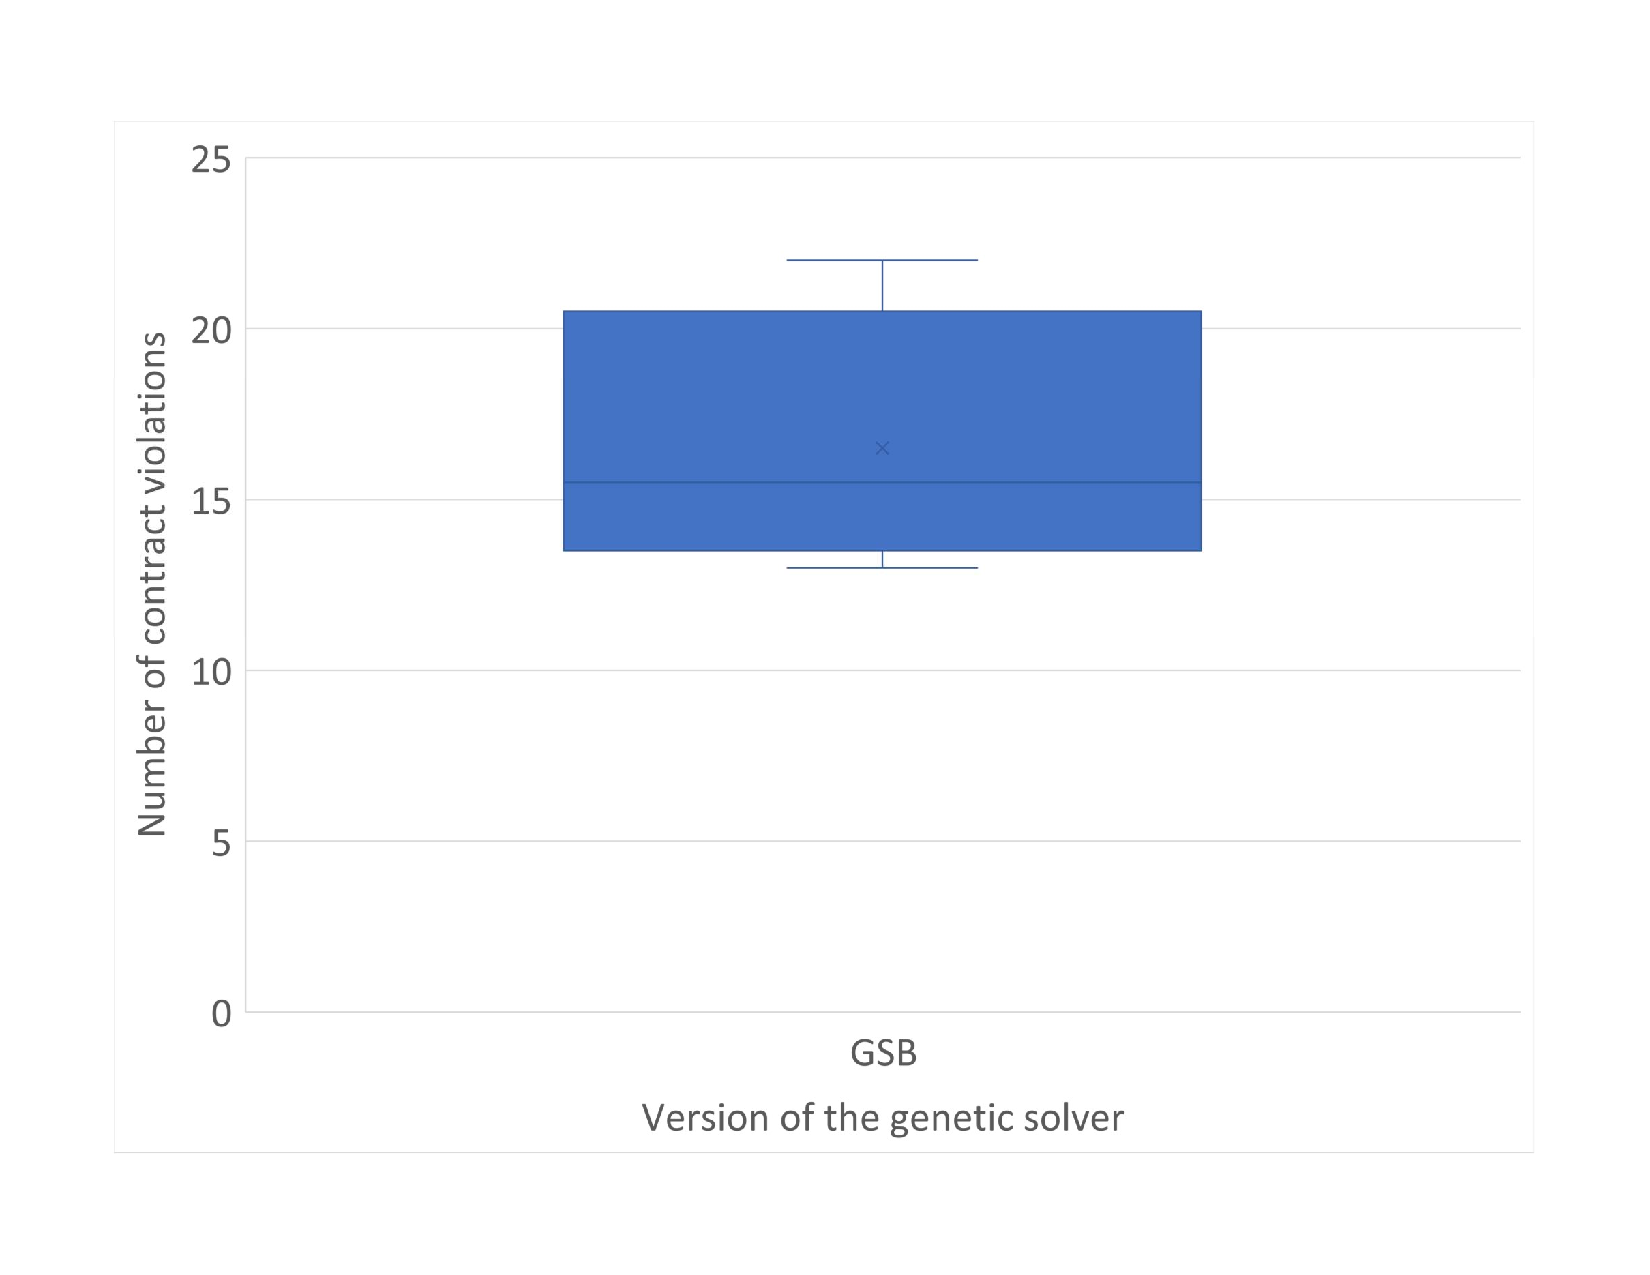
\includegraphics[width=\textwidth]{images/BoxPlotSolverBasic}
	\caption[Boxplot with a number of contract violations for the basic version of genetic solver]{}
	\label{fig:boxplotsolverbasic}
\end{figure}


\section{Parameters that need tuning}
The first step to improve the genetic solver was a parameter optimization. To perform parameter optimization was performed a few important steps.
\begin{enumerate}
	\item Analysis of genetic solver to find out all parameters that could be changed. 
	\item Adapt BRISE to work with the genetic solver.
	\item Prepare Experiment description for BRISE.
	\item Run BRISE to get the optimal configuration.
\end{enumerate}

After deep-diving into the code of genetic solver, the list of parameters was prepared.
In the basic version of the genetic solver, there are only three parameters that are changeable on call. There are:
\begin{itemize}
	\item selectorType - type of the selector algorithm that was mentioned in section~\ref{sec:GeneticAlgorithm:Selector},
	\item Number of generation - number of generations that performed by the genetic solver, working as a termination condition, in this thesis we use only timeout termination, so this parameter set as a huge value,
	\item PopulationSize - number of individuals in a population.
\end{itemize}

Adaptation of genetic solver to work into a BRISE consist of a few steps:
\begin{enumerate}
	\item prepare executable file of genetic solver,
	\item implement a method for a worker that will call the file from the previous step and returns the results with a number of contract violations and energy consumption.
\end{enumerate}

Step number 3 means that the user describes parameters that need to optimize, their names, ranges if the parameter has continuous range, or all variants if categorical. The user also should set what components to use, what the minimal number of measurements of a single Configuration, etc.
For parameter optimization of genetic solver, we use the experiment description shown in \todo{appendix or here?}.
\begin{table}
	\begin{tabularx}{\textwidth}{@{}rrrrrrrrrrrr@{}}
		\toprule
		\textbf{selectorType} & \textbf{PopulationSize} &
		\textbf{lambda} & \textbf{CrossoverRate} & \textbf{mu} & \textbf{MutationRate} 
		 & \textbf{ResourceMutationProbability}  & \textbf{CrossoverProbability}  & \textbf{ValidityWeight} & \textbf{SoftwareValidityWeight} & \textbf{RandomSoftwareAssignmentAttempts}
		 & \textbf{populateSoftwareSolutionAttempts}
		\tabularnewline
		\midrule
		1 & 1.23 & 0.01 & 0 & 0 & 0 & 0 & 0 & 0 & 0 & 0 & 0
		\tabularnewline
		1 & 1.23 & 0.01 & 0 & 0 & 0 & 0 & 0 & 0 & 0 & 0 & 0
		\tabularnewline
		\bottomrule
	\end{tabularx}
	\caption{Table name}\label{tab:EnergyTable}
\end{table}
When optimal configuration was founded, we use it to analyze results in a boxplot.
The results showed on Figure~\ref{fig:boxplotsolverbasictuning}.
\begin{figure}
	\centering
	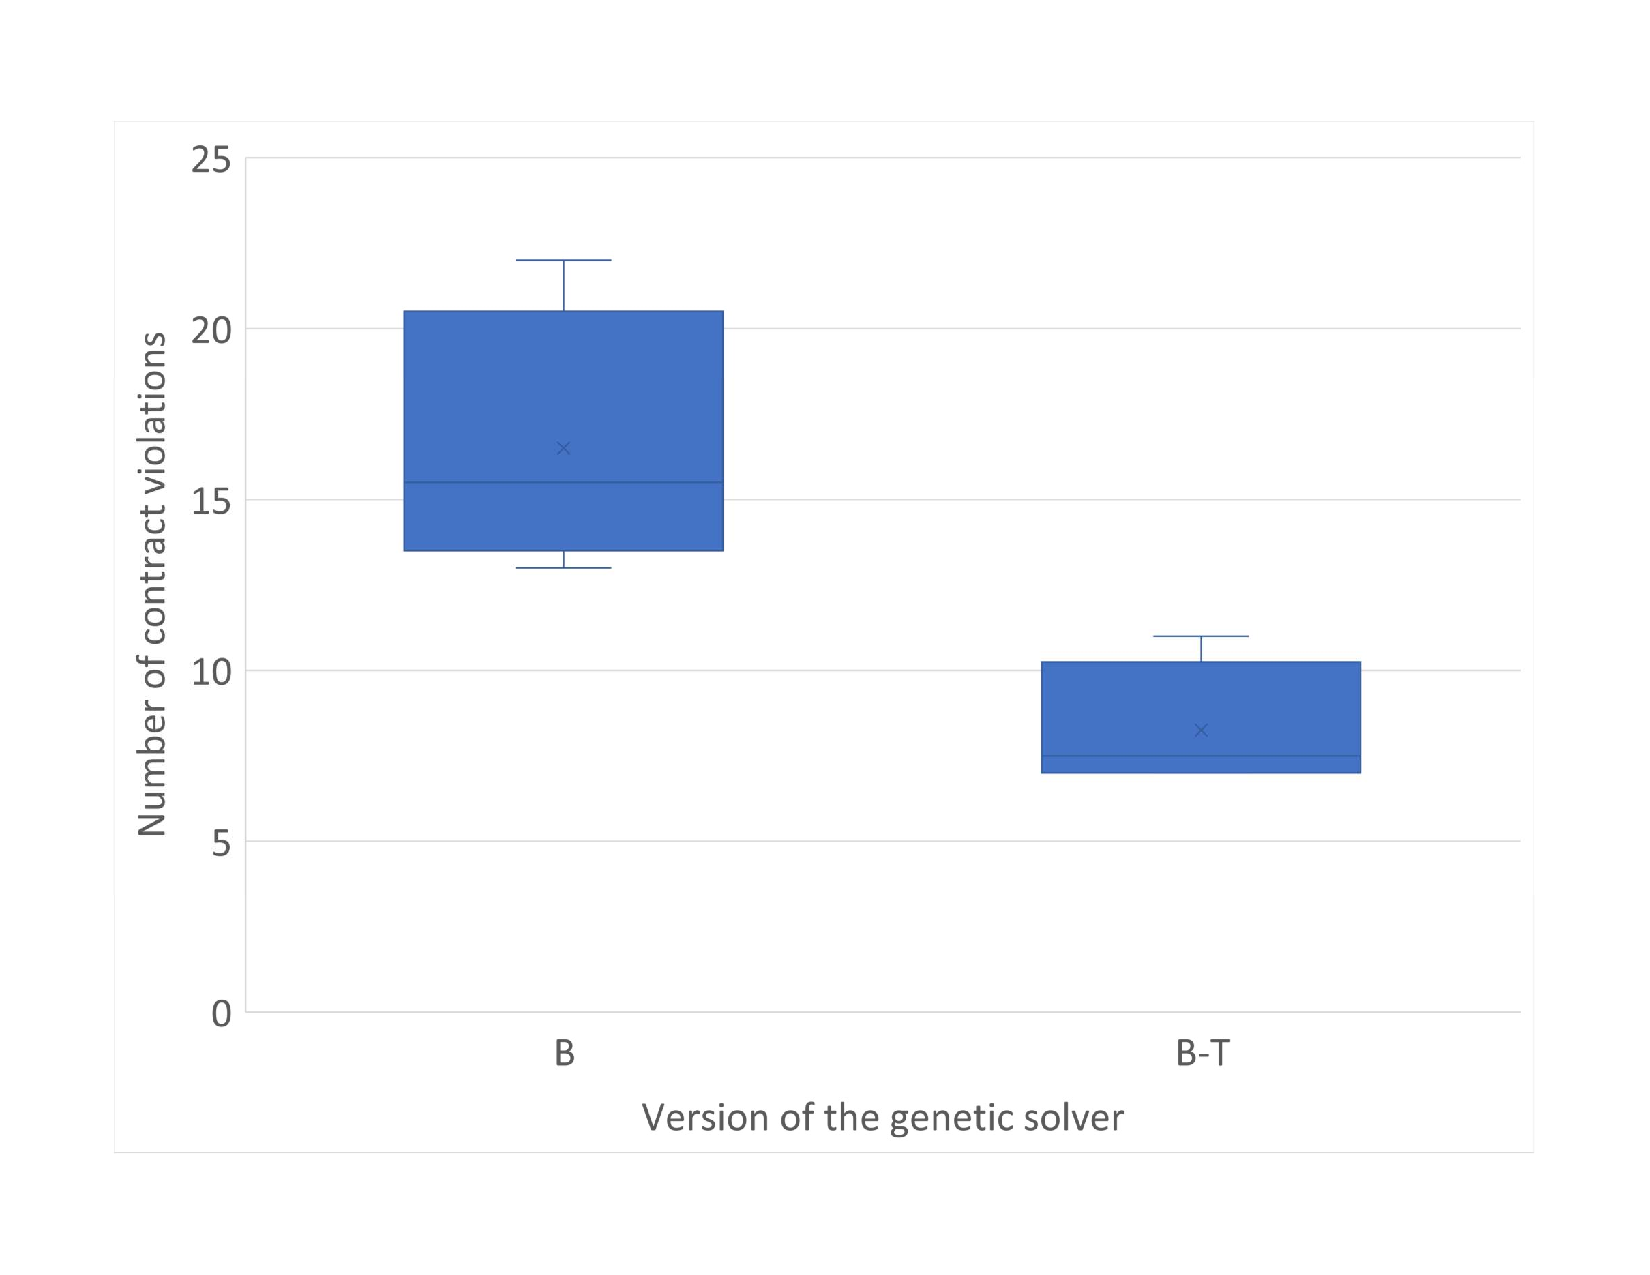
\includegraphics[width=\textwidth]{images/BoxPlotSolverBasicTuning}
	\caption[Boxplot with a number of contract violations for the basic version of genetic solver and with tuned parameters]{}
	\label{fig:boxplotsolverbasictuning}
\end{figure}

Conclusions of this step:
\begin{enumerate}
	\item All results still not valid.
	\item Number of contract violations is less.
	\item The distance between max and min result is smaller.
\end{enumerate}
Here we get the answer on \textbf{RQ2}: parameter tuning has an affect on the results of the genetic solver.

\section{More parameters}
The previous section shows that even with a good set of parameters, a genetic solver could not get valid results.
After more detailed analysis of code, we found out more parameters, that are not exposed for external tuning:
	 \paragraph{\texttt{lambda}} - as mentioned in section~\ref{sec:GeneticAlgorithm:Selecto}, it describes the number of new offspring per generation. In this step it was changed to a part of population size,
	 \paragraph{\texttt{CrossoverRate}} - as mentioned in section~\ref{sec:GeneticAlgorithmCrossover}, it describes the probability of two individuals to exchange their genes,
	 \paragraph{\texttt{mu}} - as mentioned in section~\ref{sec:GeneticAlgorithm:Selecto}, it describes the number of parents, selected by the selector to create new individuals. In this step it was changed to a part of population size,
	 \paragraph{\texttt{MutationRate}} - as mentioned in section~\ref{sec:GeneticAlgorithmMutation}, it describes the probability of the individual to mutate,
	 \paragraph{\texttt{ResourceMutationProbability}} - the probability that during mutation mapped resource will mutate,
	 \paragraph{\texttt{CrossoverProbability}} - probability to do crossover inside crossover operator. This parameter was removed in later versions of the genetic solver, because it duplicate the functionality of \texttt{CrossoverRate} And this fact gives the answer on \textbf{RQ1}. There is a bad decision in the genetic solver.
	 
	 
	 \paragraph{\texttt{ValidityWeight}} - coefficient that shows how each contract violation degrees the quality of the solution, 
	 \paragraph{\texttt{SoftwareValidityWeight}} - coefficient that shows how each error in software tree degrees the quality of the solution,
	 \paragraph{\texttt{RandomSoftwareAssignmentAttempts}} - max number of attempts to set a valid software tree to the individual on the creation phase,
	 \paragraph{\texttt{populateSoftwareSolutionAttempts}} -  max number of attempts to assign software components and resources to get a valid individual on the creation phase.

To make them changeable, we use \texttt{GoogleGuiceDependencyInjection}\footnote{\url{https://github.com/google/guice}} to change the values of these parameters during the solver call.

\begin{table}
	\begin{tabularx}{\textwidth}{@{}rrrrrrrrrrrr@{}}
		\toprule
		\textbf{selectorType} & \textbf{PopulationSize} &
		\textbf{lambda} & \textbf{CrossoverRate} & \textbf{mu} & \textbf{MutationRate} 
		& \textbf{ResourceMutationProbability}  & \textbf{CrossoverProbability}  & \textbf{ValidityWeight} & \textbf{SoftwareValidityWeight} & \textbf{RandomSoftwareAssignmentAttempts}
		& \textbf{populateSoftwareSolutionAttempts}
		\tabularnewline
		\midrule
		1 & 1.23 & 0.01 & 0 & 0 & 0 & 0 & 0 & 0 & 0 & 0 & 0
		\tabularnewline
		\bottomrule
	\end{tabularx}
	\caption{Table name}\label{tab:EnergyTable}
\end{table}

Figure~\ref{fig:boxplotsolverNoHardcodedTuning} shows the results of genetic solver with all parameters after optimization in BRISE.
\begin{figure}
	\centering
	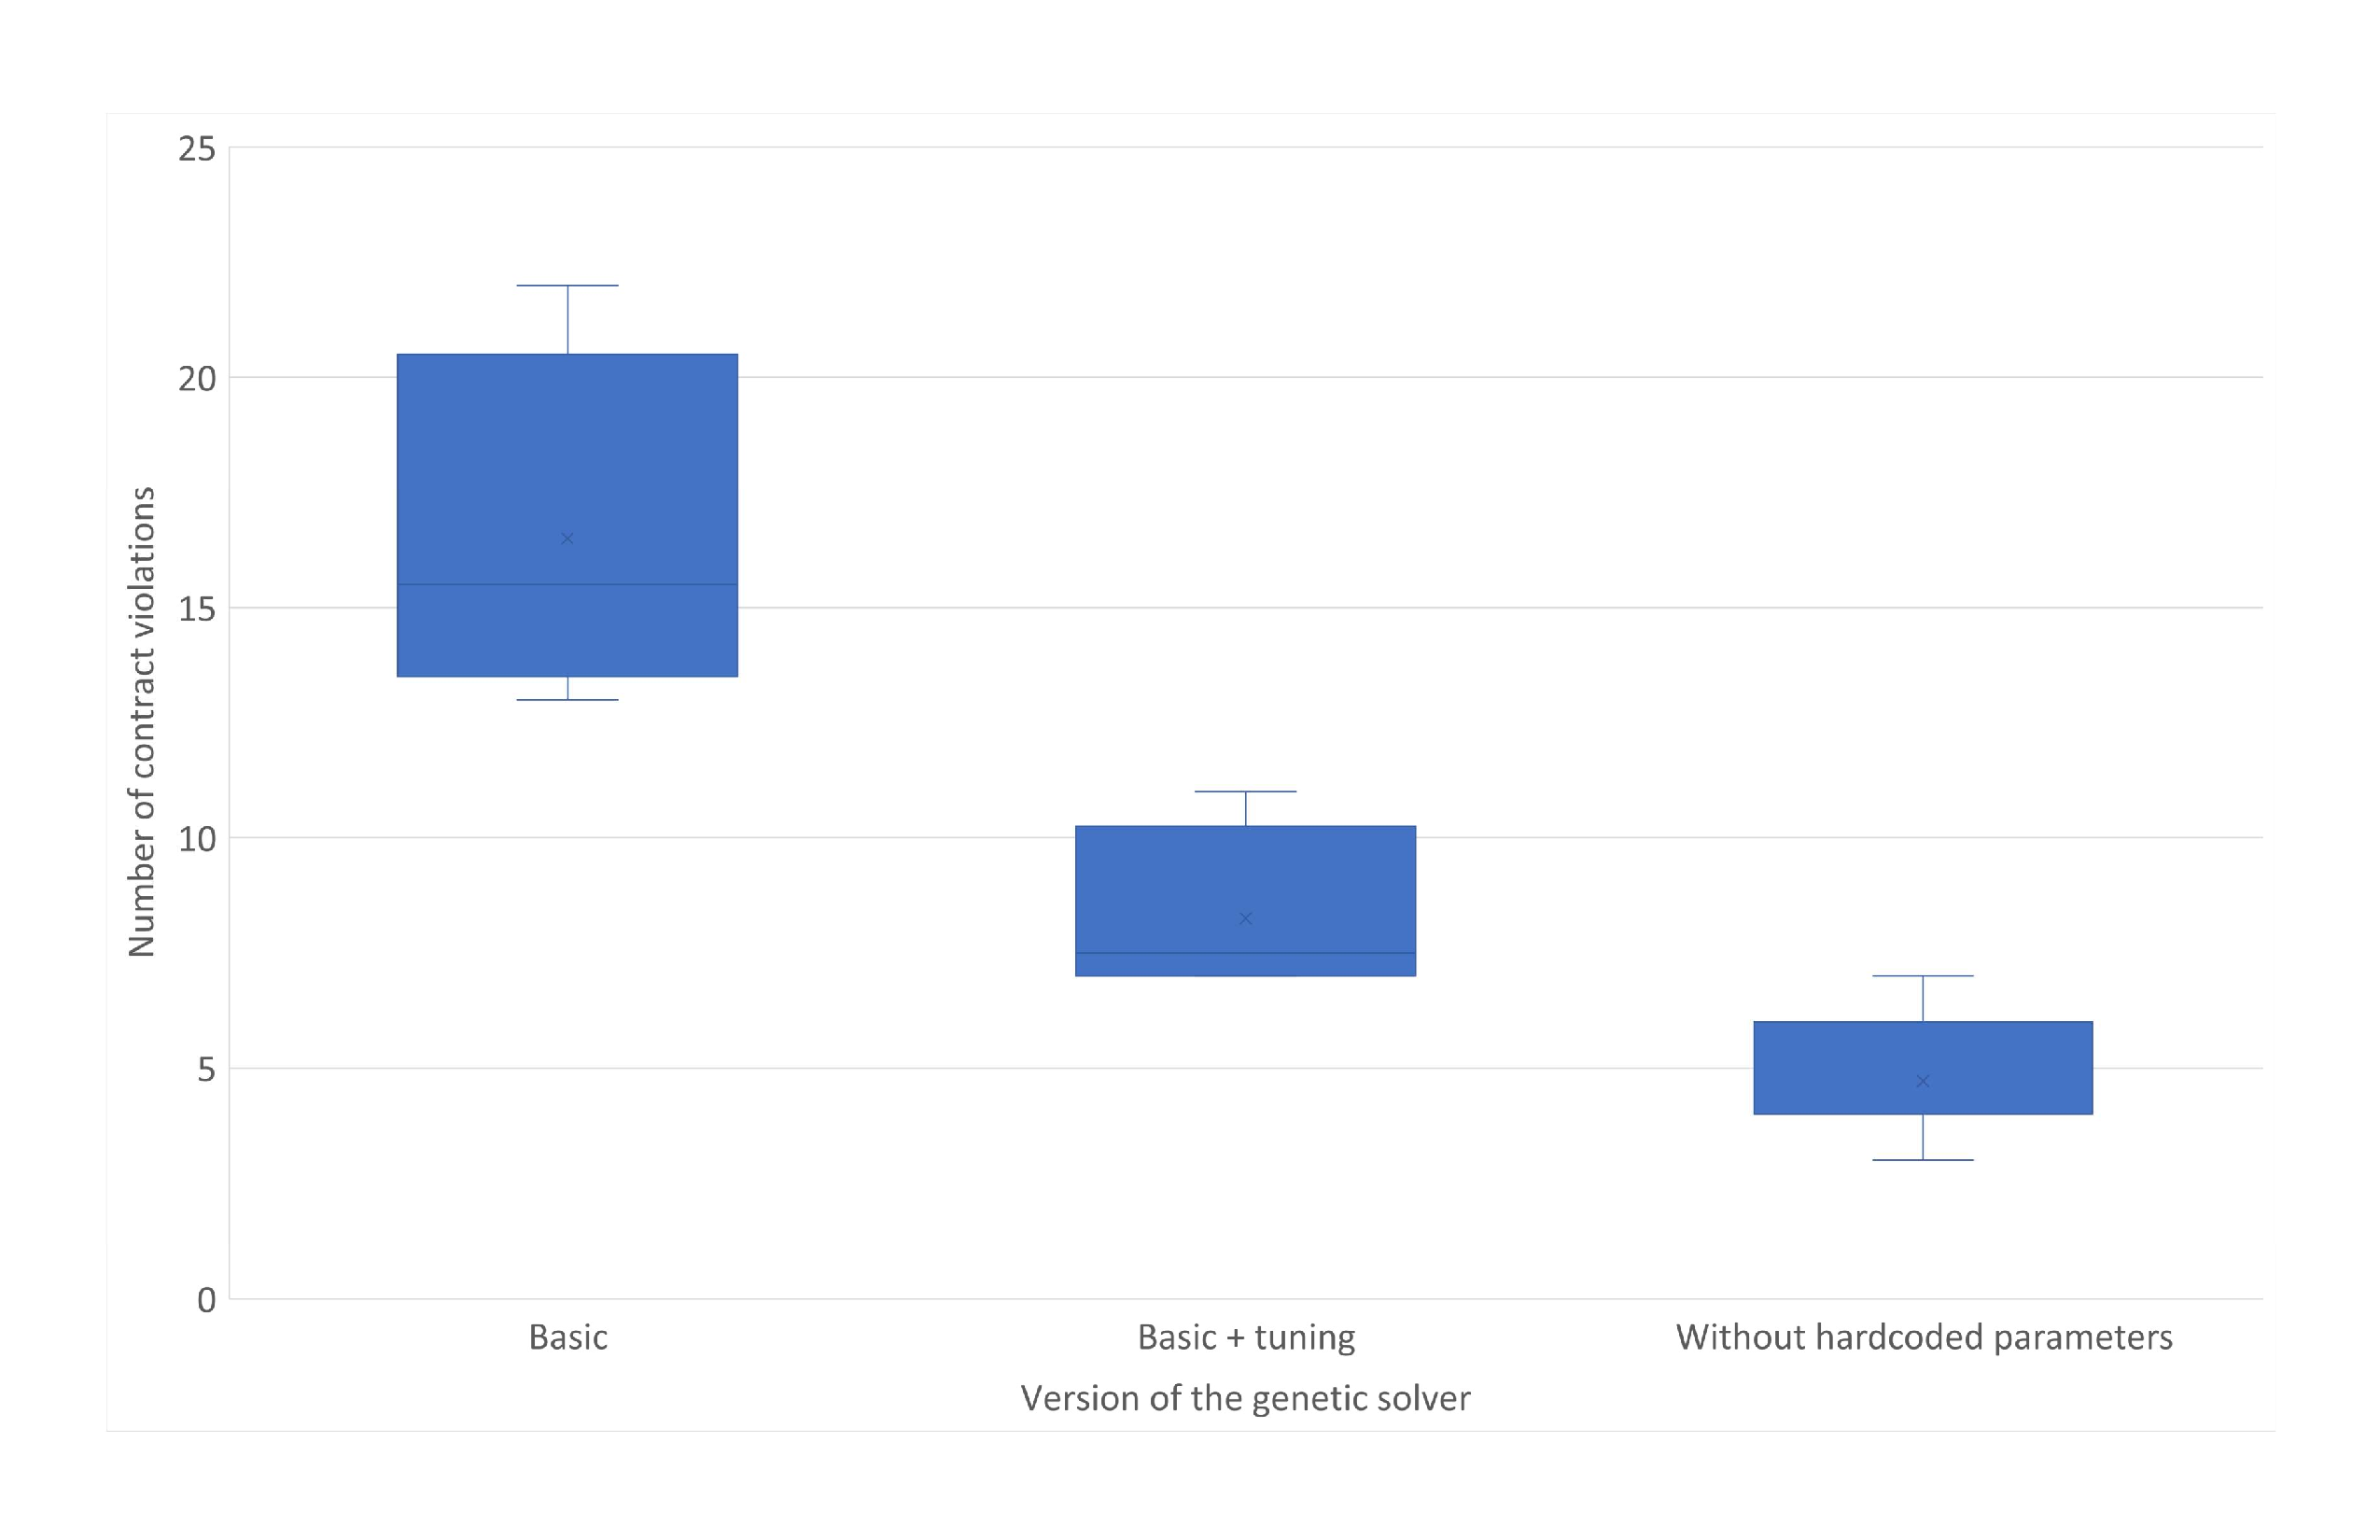
\includegraphics[width=\textwidth]{images/BoxPlotSolverNoHardcodedTuning.pdf}
	\caption[Boxplot with a number of contract violations for the genetic solver without hardcoded parameters in comparison with previous versions]{Boxplot with a number of contract violations for the genetic solver without hardcoded parameters in comparison with previous versions}
	\label{fig:boxplotsolverNoHardcodedTuning}
\end{figure}
Results a bit better but still without valid results.
This step confirms the fact that good values of parameters have a significant influence on the results, but sometimes parameter tuning not enough to get good results. 

\section{Even more parameters}
Due to fact, that parameter tuning from previous step could not give a valid results, we decide to use another approach called parameter engineering.
Detailed analysis of crossover and mutation operators showed that crossover point and mutation points are coarse-grained.

The crossover point is defined as a node of the tree shape genotype recursively comparing the corresponding nodes of the threes by software implementation and the hardware resource for each request.
If it is not located at the root of the tree, then the exchange occurs with all children.

Mutation point is defined for one random request, and with probability `MutationRate`, it mutates the root of the tree shape genotype otherwise both children.

We add a few more probabilities to crossover and mutation operators. These probabilities allow to change location of crossover/mutation points in different ways of the Tree Shape Genotype.
There are:
	\paragraph{\texttt{CrossoverOnRandomChildProbability}} - chance that crossover will occur on the random child, or on both children otherwise,
	\paragraph{\texttt{CrossoverOnRandomLevelProbability}} - the probability that describes a chance to do a crossover on random level of the tree, 
	\paragraph{\texttt{CrossoverOnRandomRequestProbability}} - a chance to do a crossover on random request,
	\paragraph{\texttt{MutationOnRandomChildProbability}} - the probability that describes a chance of mutation on a random child,
	\paragraph{\texttt{MutationOnRandomLevelProbability}} - the chance of mutation on a random level of the tree shape genotype.

\begin{table}
	\begin{tabularx}{\textwidth}{@{}rrrrrrrrrrrrrrrrr@{}}
		\toprule
		\textbf{selectorType} & \textbf{PopulationSize} &
		\textbf{lambda} & \textbf{CrossoverRate} & \textbf{mu} & \textbf{MutationRate} 
		& \textbf{ResourceMutationProbability}  & \textbf{CrossoverProbability}  & \textbf{ValidityWeight} & \textbf{SoftwareValidityWeight} & \textbf{RandomSoftwareAssignmentAttempts}
		& \textbf{populateSoftwareSolutionAttempts} & \textbf{CrossoverOnRandomChildProbability}
		& \textbf{CrossoverOnRandomLevelProbability} & \textbf{CrossoverOnRandomRequestProbability}
		& \textbf{MutationOnRandomChildProbability} & \textbf{MutationOnRandomLevelProbability}
		\tabularnewline
		\midrule
		1 & 1.23 & 0.01 & 0 & 0 & 0 & 0 & 0 & 0 & 0 & 0 & 0 & 0 & 0 & 0 & 0 & 0
		\tabularnewline
		1 & 1.23 & 0.01 & 0 & 0 & 0 & 0 & 0 & 0 & 0 & 0 & 0 & 0 & 0 & 0 & 0 & 0
		\tabularnewline
		\bottomrule
	\end{tabularx}
	\caption{Table name}\label{tab:EnergyTable}
\end{table}

After those probabilities were added to operators with some default values of probabilities and all previous parameters were as in basic version, the results of the genetic solver were almost the same as results from the previous section (Figure~\ref{fig:boxplotsolverNewParameters}).
\begin{figure}
	\centering
	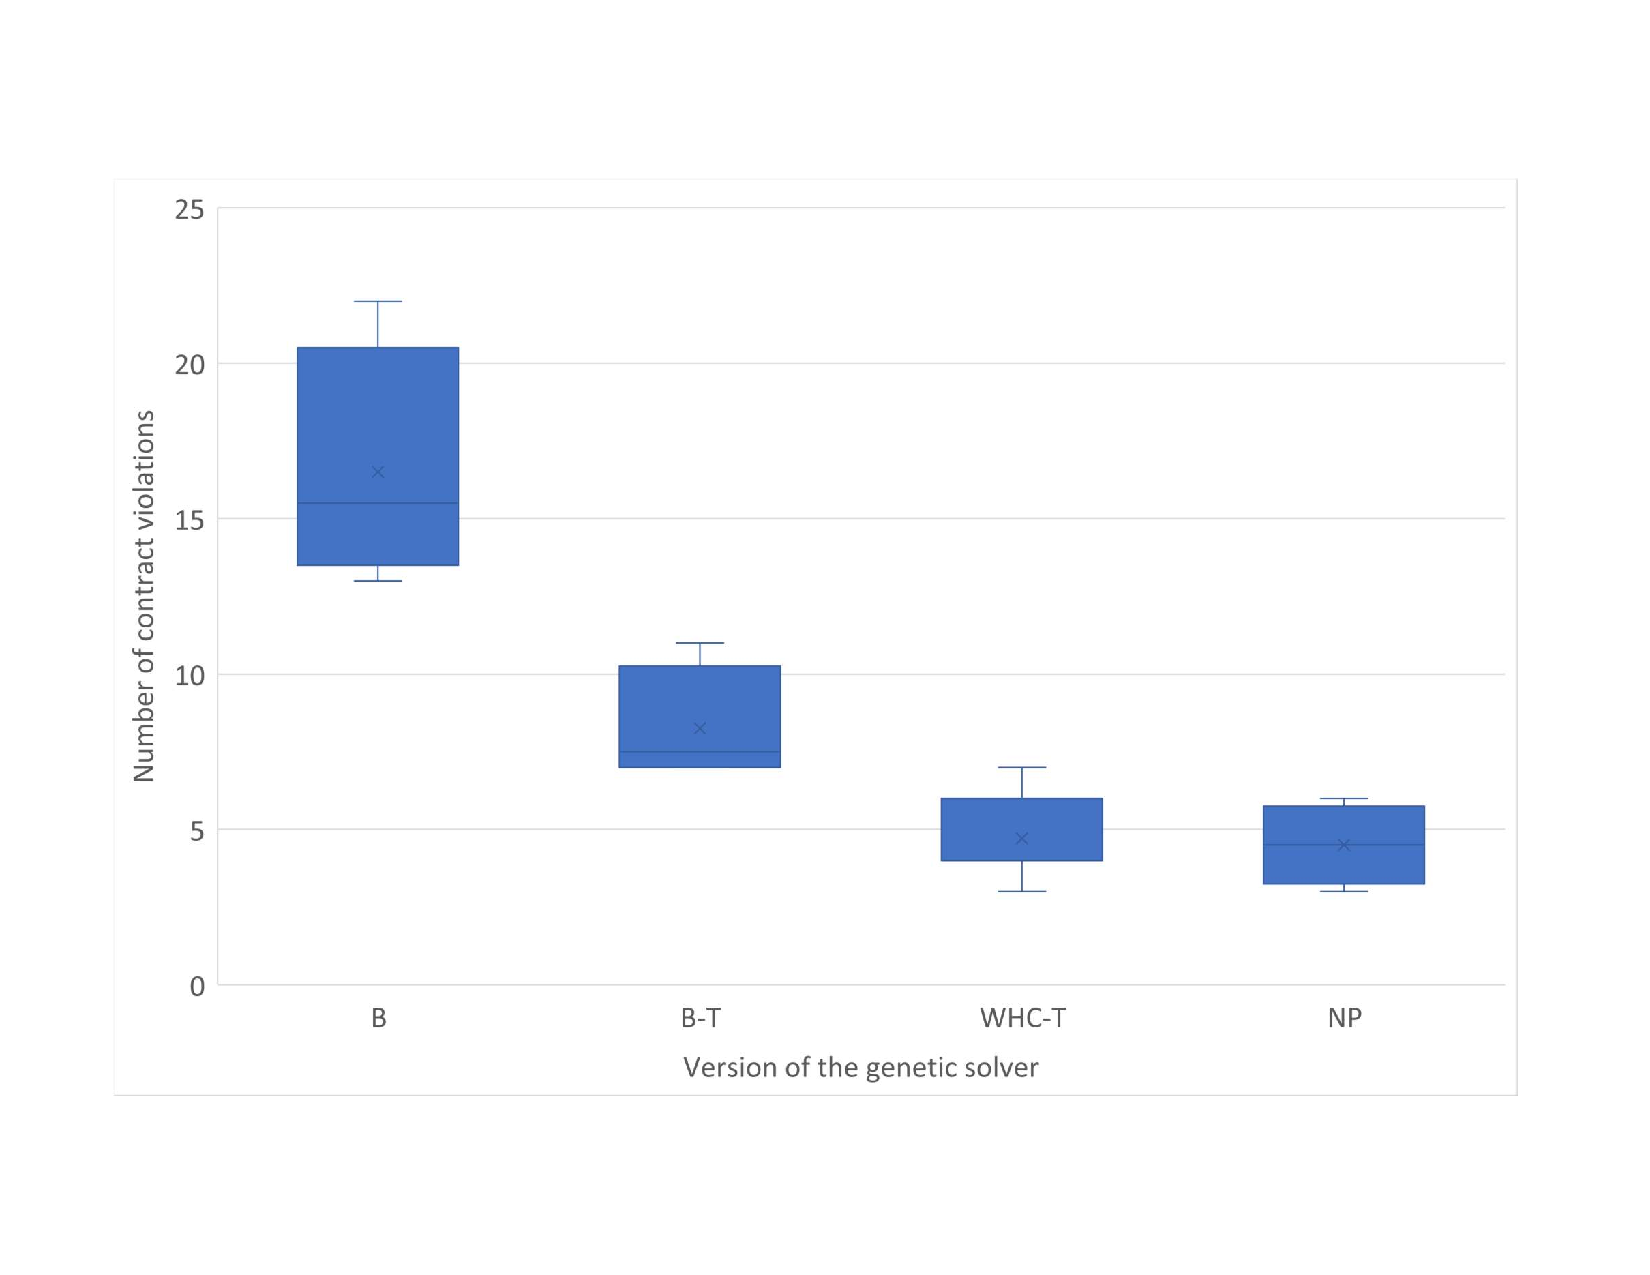
\includegraphics[width=\textwidth]{images/BoxPlotSolverNewParameters.pdf}
	\caption[Boxplot with a number of contract violations for the genetic solver with added probabilities without tuning in comparison with previous versions]{Boxplot with a number of contract violations for the genetic solver with added probabilities without tuning in comparison with previous versions}
	\label{fig:boxplotsolverNewParameters}
\end{figure}

These results show that new parameters have a big influence on the result of tuning. That means that good parameter engineering is important in any process.  But what if we could tune new parameters together with others?
Figure~\ref{fig:boxplotsolverNewParametersTuning} shows the result that combine new probabilities and parameter tuning.
\begin{figure}
	\centering
	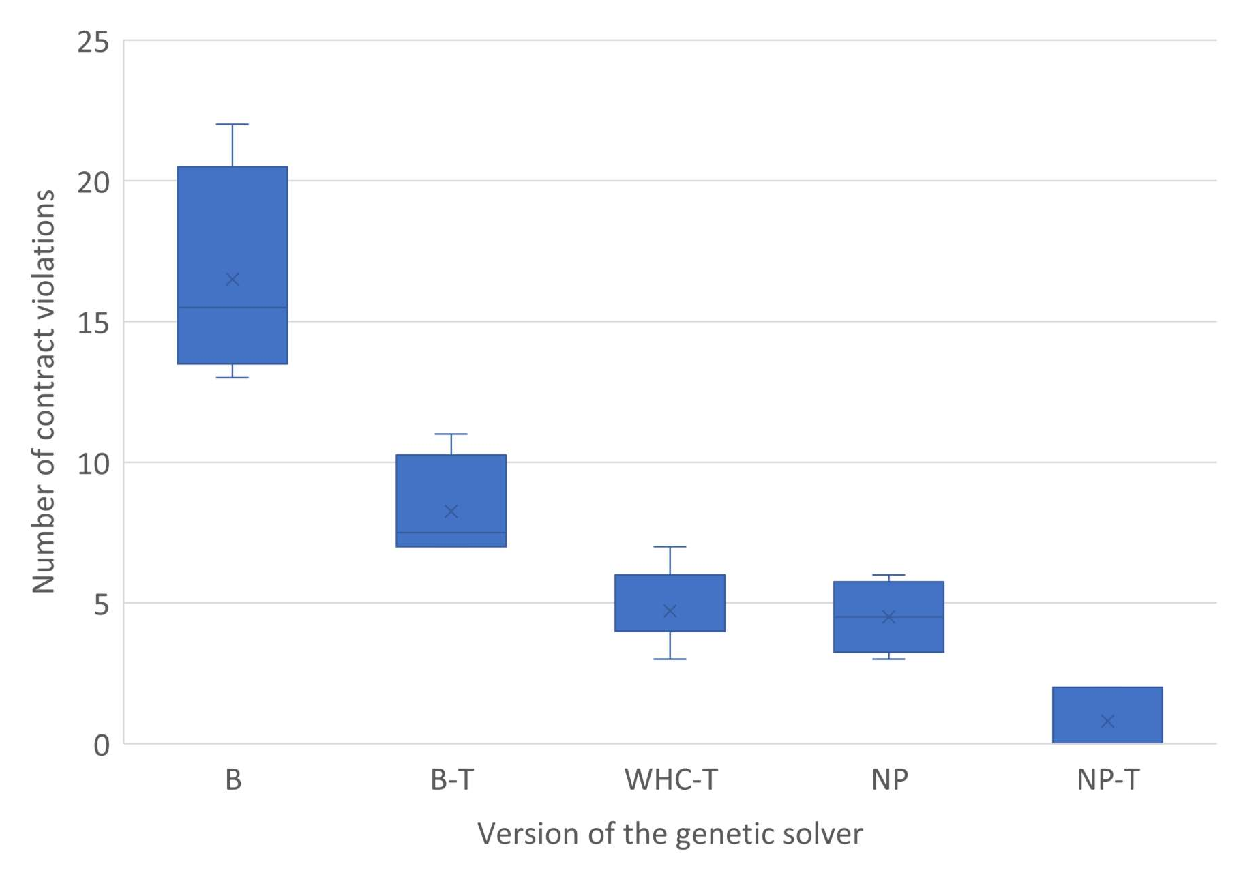
\includegraphics[width=\textwidth]{images/BoxPlotSolverNewParametersTuning.pdf}
	\caption[Boxplot with a number of contract violations for the genetic solver with added probabilities and tuned parameters in comparison with previous versions]{Boxplot with a number of contract violations for the genetic solver with added probabilities and tuned parameters in comparison with previous versions}
	\label{fig:boxplotsolverNewParametersTuning}
\end{figure}

The combined approach of new parameters and parameter tuning gives a valid result. The boxplot also shows that not all results are valid. The reason for this is the local optimum and the inability to get out of it due to the fact that at a certain moment, the majority of the individual in the population becomes the same. 

\section{Adaptive parameters}
The reason why all individuals in the population are the same is primarily due to the crossover. To create new individuals, the selector takes the best individuals. Crossover, taking two individuals, and performing a gene change, creates two new individuals. If these individuals are worse, then the selector in the new iteration will drop them, and if they are close, they will take them to create new individuals. At a certain point, a situation occurs that the crossover occurs between two identical genotypes, which creates two the same individuals. This exponentially increases the number of identical elements and leads to the collapse of the genetic diversity of the population.

The idea of how to solve this issue is an adaptive crossover rate that changes the chance of the crossover depends on the number of the same individuals in a population. 
The principle of operation is as follows. After each iteration, a part of the unique genotypes in the population is calculated. If the resulting number is small, then the probability of a crossover increases, and vice versa, the probability of a crossover decreases with a small number of unique individuals.

\begin{table}
	\begin{tabularx}{\textwidth}{@{}rrrrrrrrrrrrrrrrrrr@{}}
		\toprule
		\textbf{selectorType} & \textbf{PopulationSize} &
		\textbf{lambda} & \textbf{CrossoverRate} & \textbf{mu} & \textbf{MutationRate} 
		& \textbf{ResourceMutationProbability}  & \textbf{CrossoverProbability}  & \textbf{ValidityWeight} & \textbf{SoftwareValidityWeight} & \textbf{RandomSoftwareAssignmentAttempts}
		& \textbf{populateSoftwareSolutionAttempts} & \textbf{CrossoverOnRandomChildProbability}
		& \textbf{CrossoverOnRandomLevelProbability} & \textbf{CrossoverOnRandomRequestProbability}
		& \textbf{MutationOnRandomChildProbability} & \textbf{MutationOnRandomLevelProbability}
		& \textbf{PartOfUniqueIndividualsToStopCrossover} & \textbf{PartOfUniqueIndividualsToReturnCrossover}
		\tabularnewline
		\midrule
		1 & 1.23 & 0.01 & 0 & 0 & 0 & 0 & 0 & 0 & 0 & 0 & 0 & 0 & 0 & 0 & 0 & 0 & 0 & 0
		\tabularnewline
		1 & 1.23 & 0.01 & 0 & 0 & 0 & 0 & 0 & 0 & 0 & 0 & 0 & 0 & 0 & 0 & 0 & 0 & 0 & 0
		\tabularnewline
		\bottomrule
	\end{tabularx}
	\caption{Table name}\label{tab:EnergyTable}
\end{table}


The results of the genetic solver with added adaptive crossover rate with a basic set of parameters and with tuned parameters showed on Figure~\ref{fig:boxplotsolverAdaptiveCrossoverTuning}
\begin{figure}
	\centering
	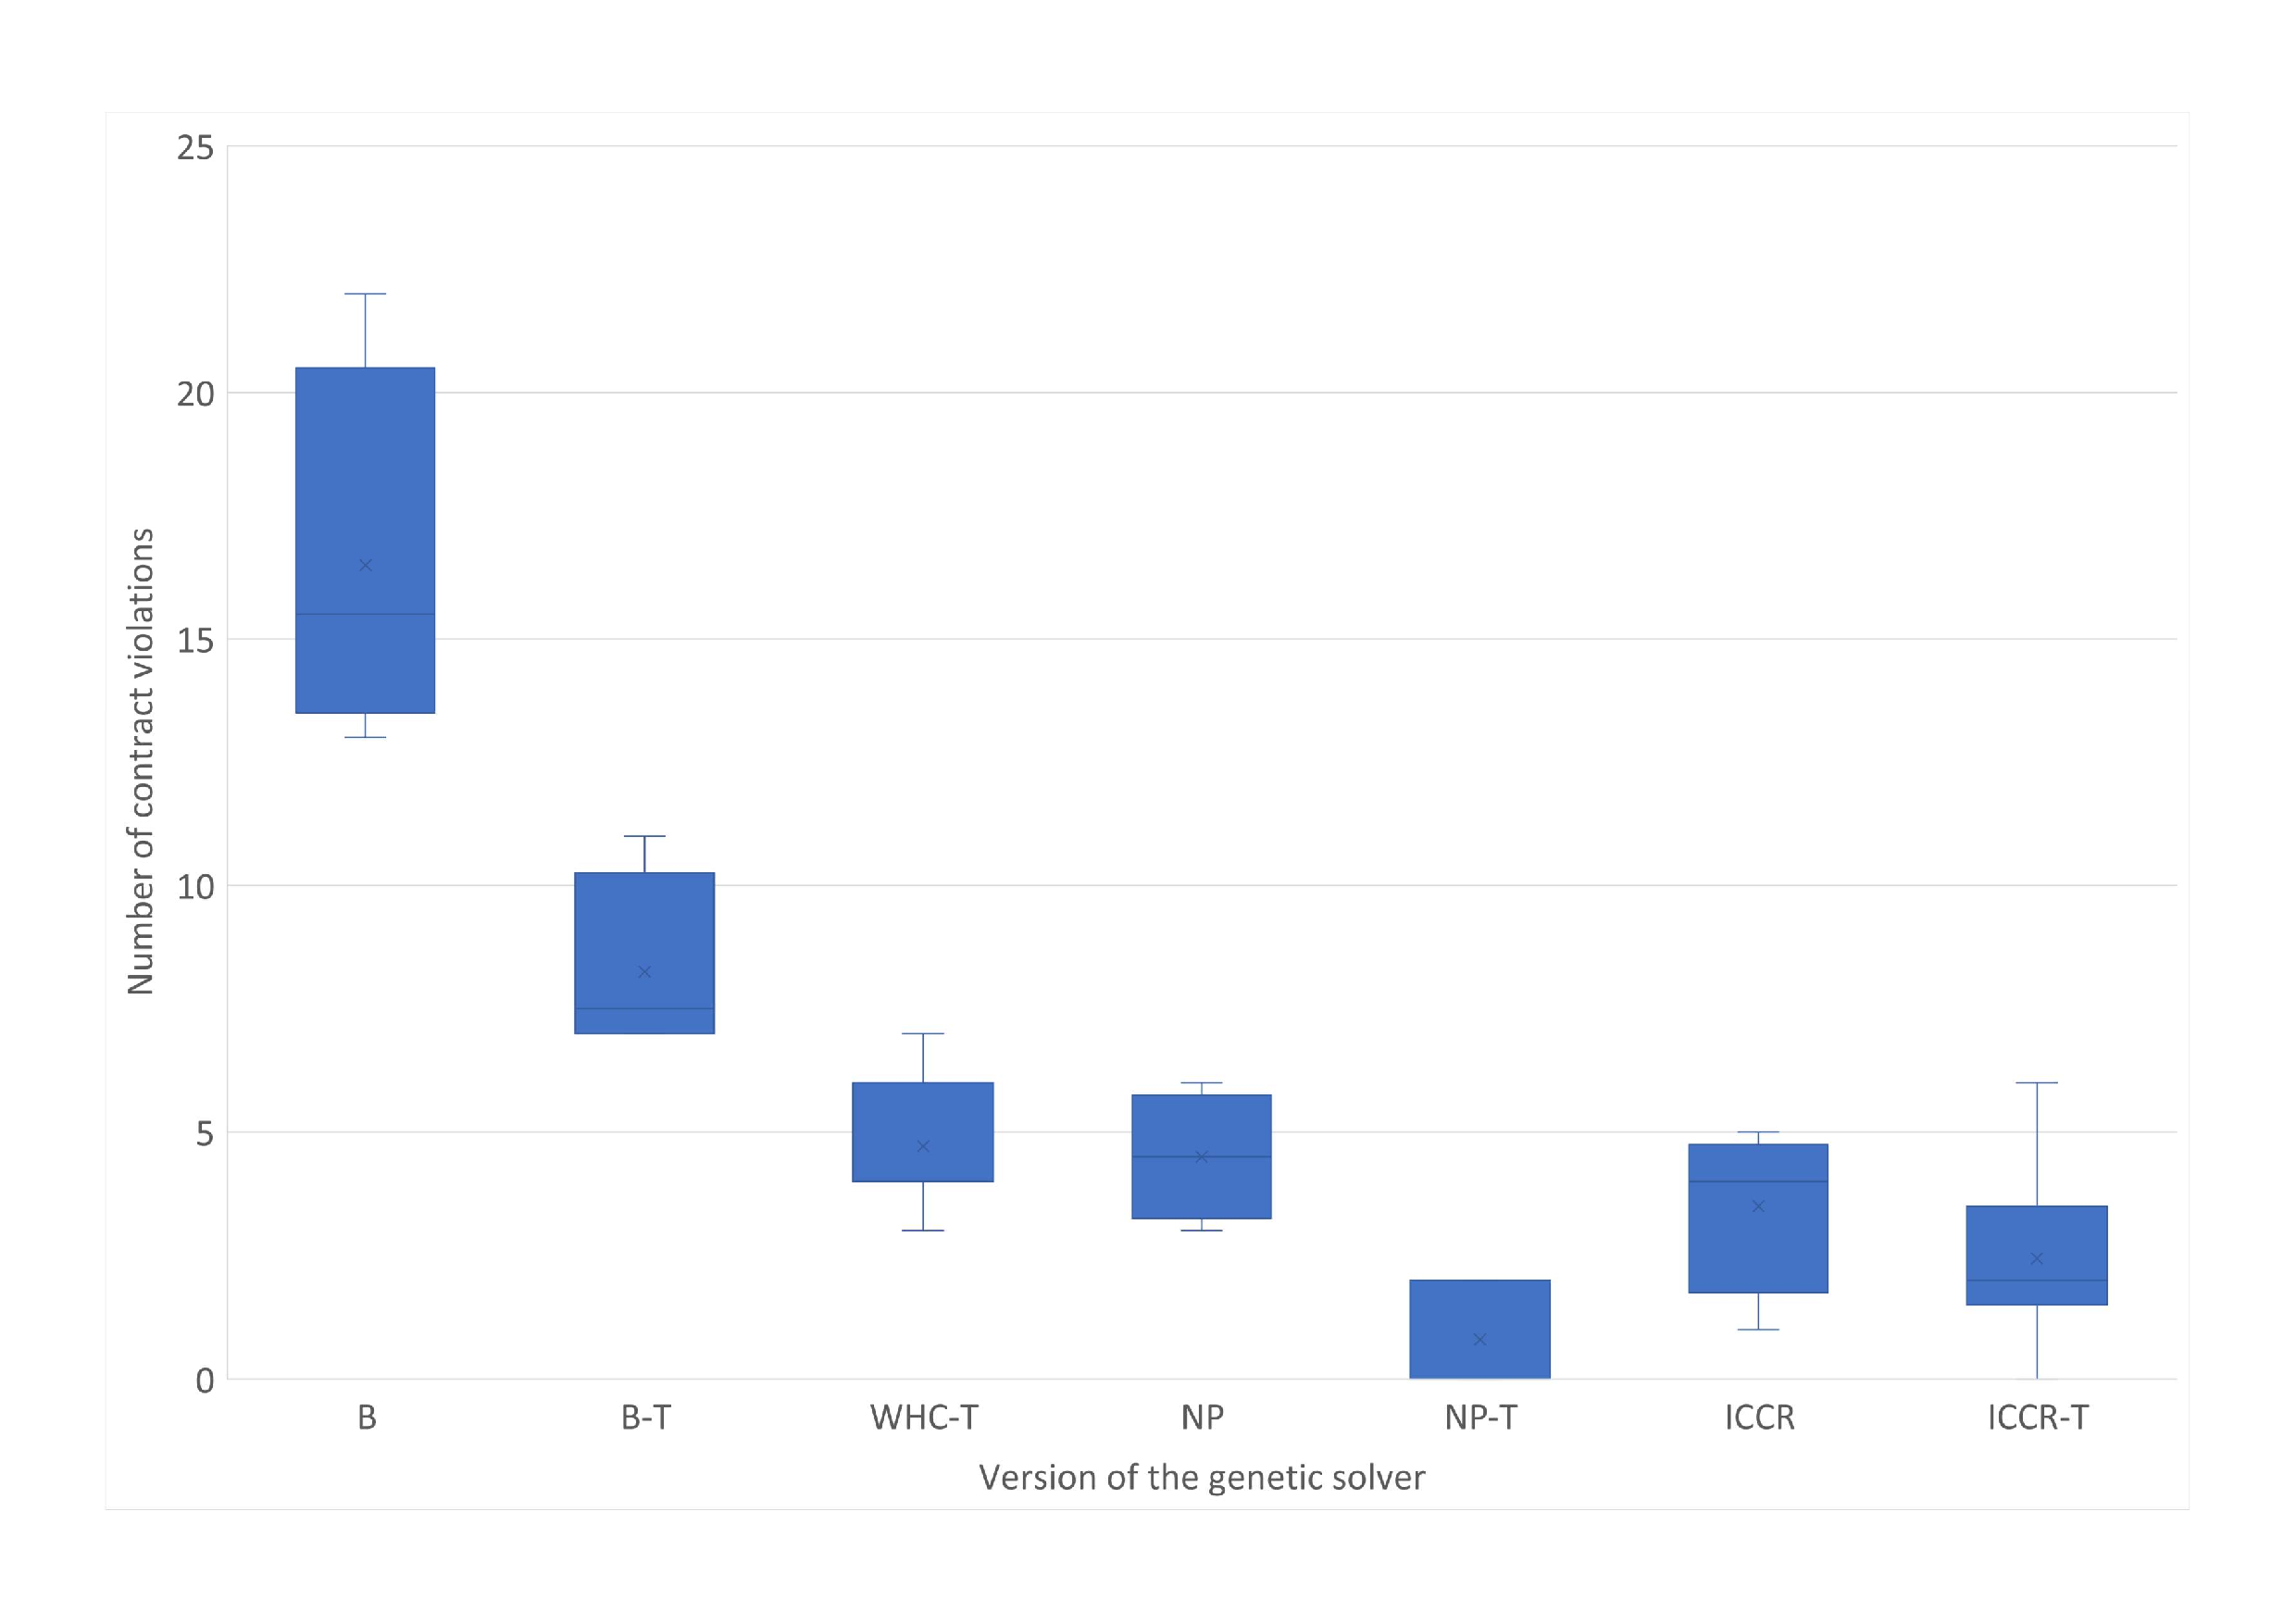
\includegraphics[width=\textwidth]{images/BoxPlotSolverAdaptiveCrossoverTuning.pdf}
	\caption[Boxplot with a number of contract violations for the genetic solver with adaptive crossover rate in comparison with previous versions]{Boxplot with a number of contract violations for the genetic solver with adaptive crossover rate in comparison with previous versions}
	\label{fig:boxplotsolverAdaptiveCrossoverTuning}
\end{figure}

As a conclusion from this section is next:
\begin{enumerate}
	\item Adaptive crossover rate gives little improvement in comparison to previous untuned versions, but results not valid.
	\item Parameter tuning works good for static parameters, but for parameters that change during the run of the genetic solver, results are worse because BRISE doesn't know that parameter could change and, most importantly, how it changes.
	\item Adaptive crossover rate helps to slightly delay the collapse of the diversity of individuals in the population, but this is not enough.
\end{enumerate} 
\begin{figure}
	\centering
	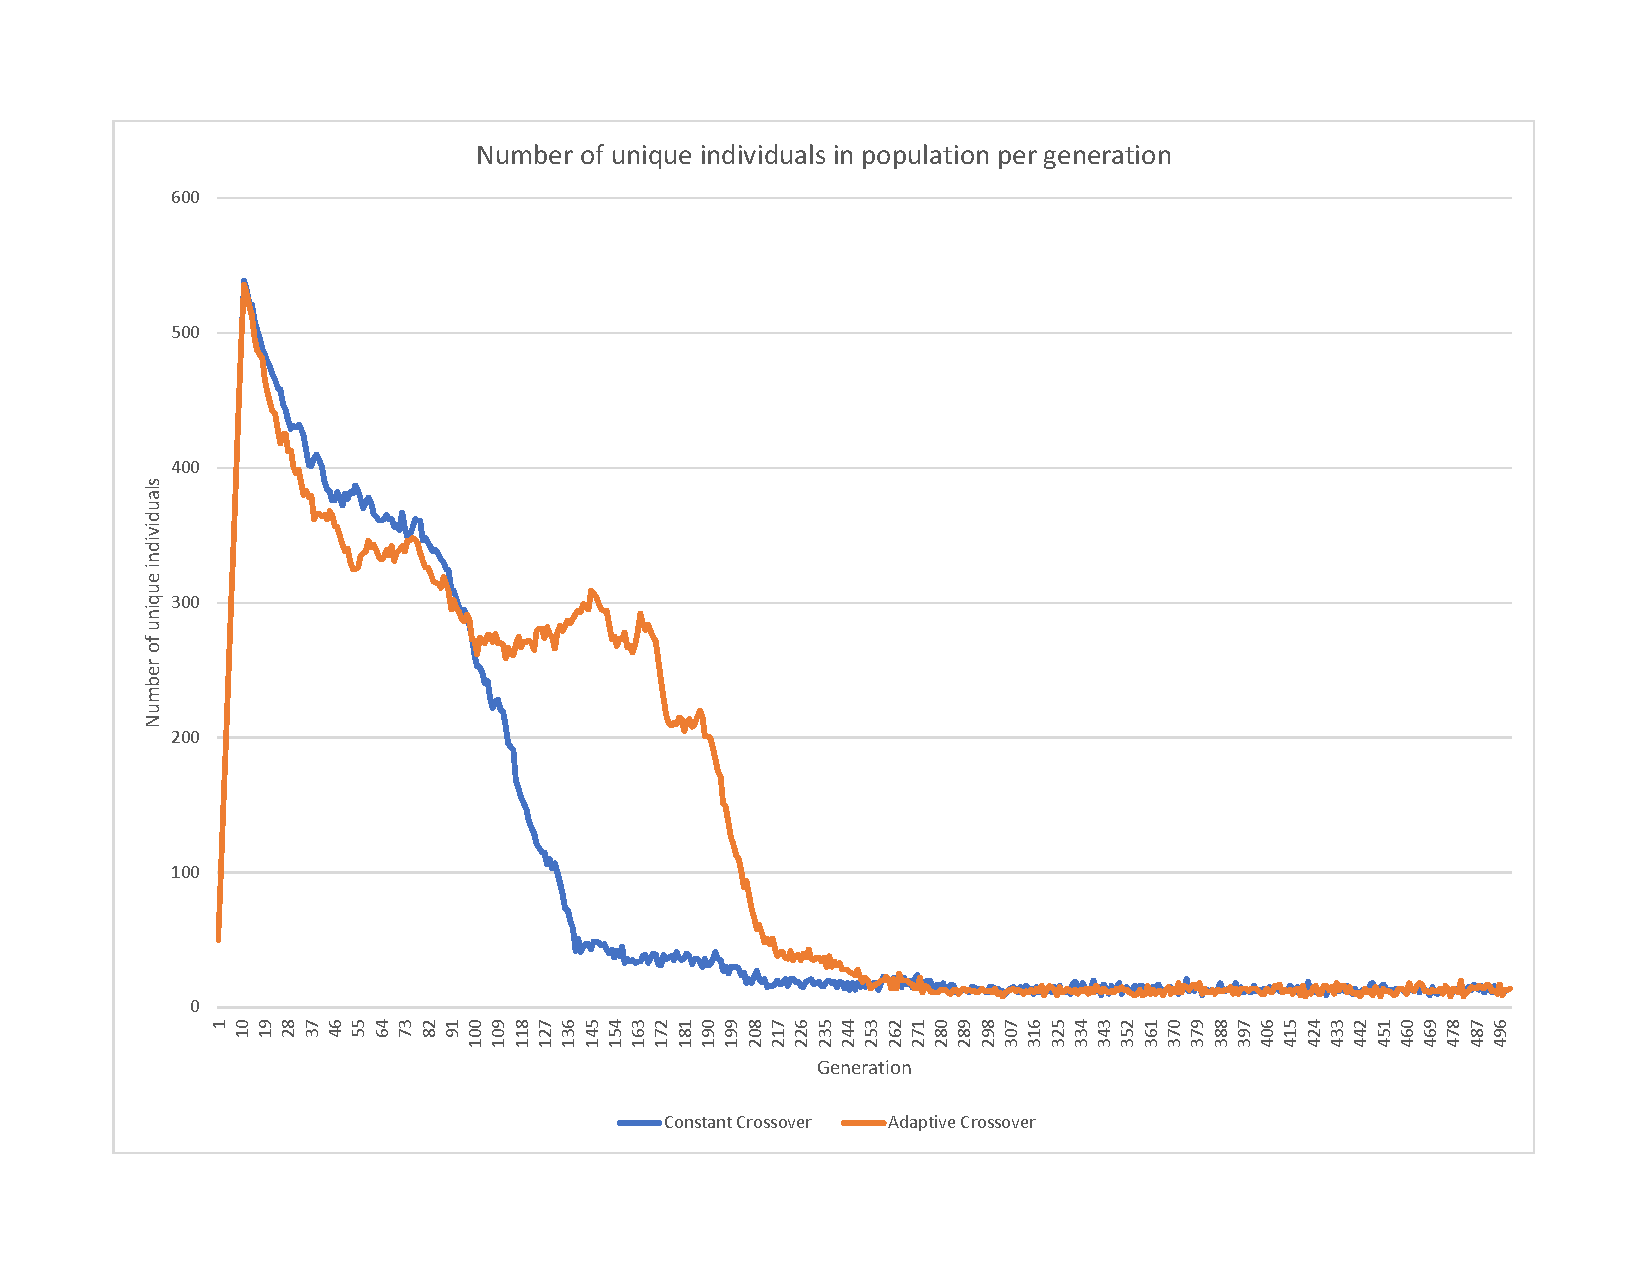
\includegraphics[width=\textwidth]{images/UniqIndividualsPerGeneration2.pdf}
	\caption[]{}
	\label{fig:UniqIndividualsPerGeneration2}
\end{figure}                        

\section{Unique genotypes in a population}
Due to the fact that the adaptive crossover did not help to reduce the number of duplicates in the population, a more radical decision was made. If the same individual already in a population, then the second one can not be added to the population. Therefore, at any moment, the population will consist of unique individuals. In this configuration of the genetic solver, the use of the adaptive crossover does not make any sense, so it was disabled, and a constant value was used.

Figure~\ref{fig:boxplotsolverNoDuplicates} shows the results of this approach without tuning and with tuned parameters. In comparison with the basic version, this approach gives better results, but in comparison with other methods described previously, the efficiency of the current approach is worth it.

The reasons for this are:
\begin{itemize}
	\item on each generation best individual could give a new offspring only a few times, 
	\item calculation speed of this approach is slower and, as a result, less generation in specified time.
\end{itemize}


\begin{figure}
	\centering
	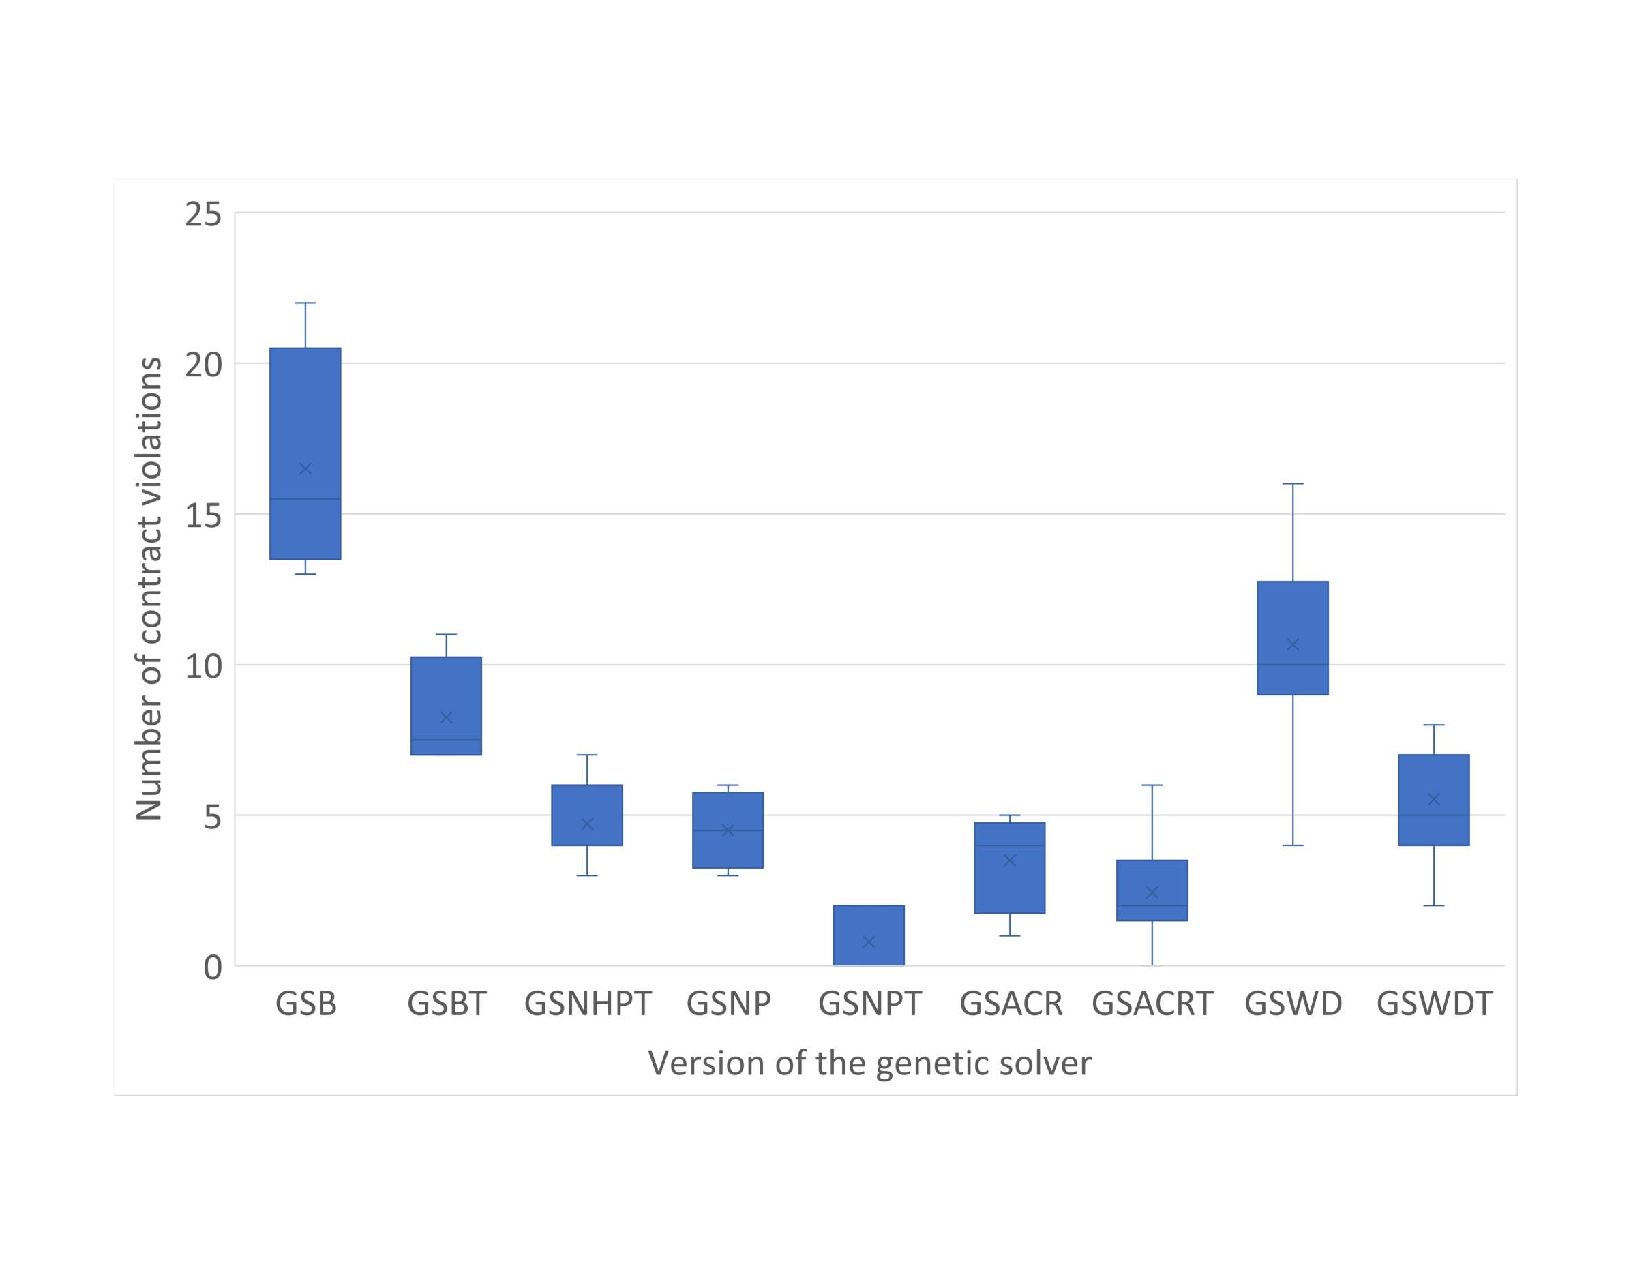
\includegraphics[width=\textwidth]{images/BoxPlotSolverNoDuplicates.pdf}
	\caption[Boxplot with a number of contract violations for the genetic solver without duplicates in the population in comparison with previous versions]{Boxplot with a number of contract violations for the genetic solver without duplicates in the population in comparison with previous versions}
	\label{fig:boxplotsolverNoDuplicates}
\end{figure}

\begin{figure}
	\centering
	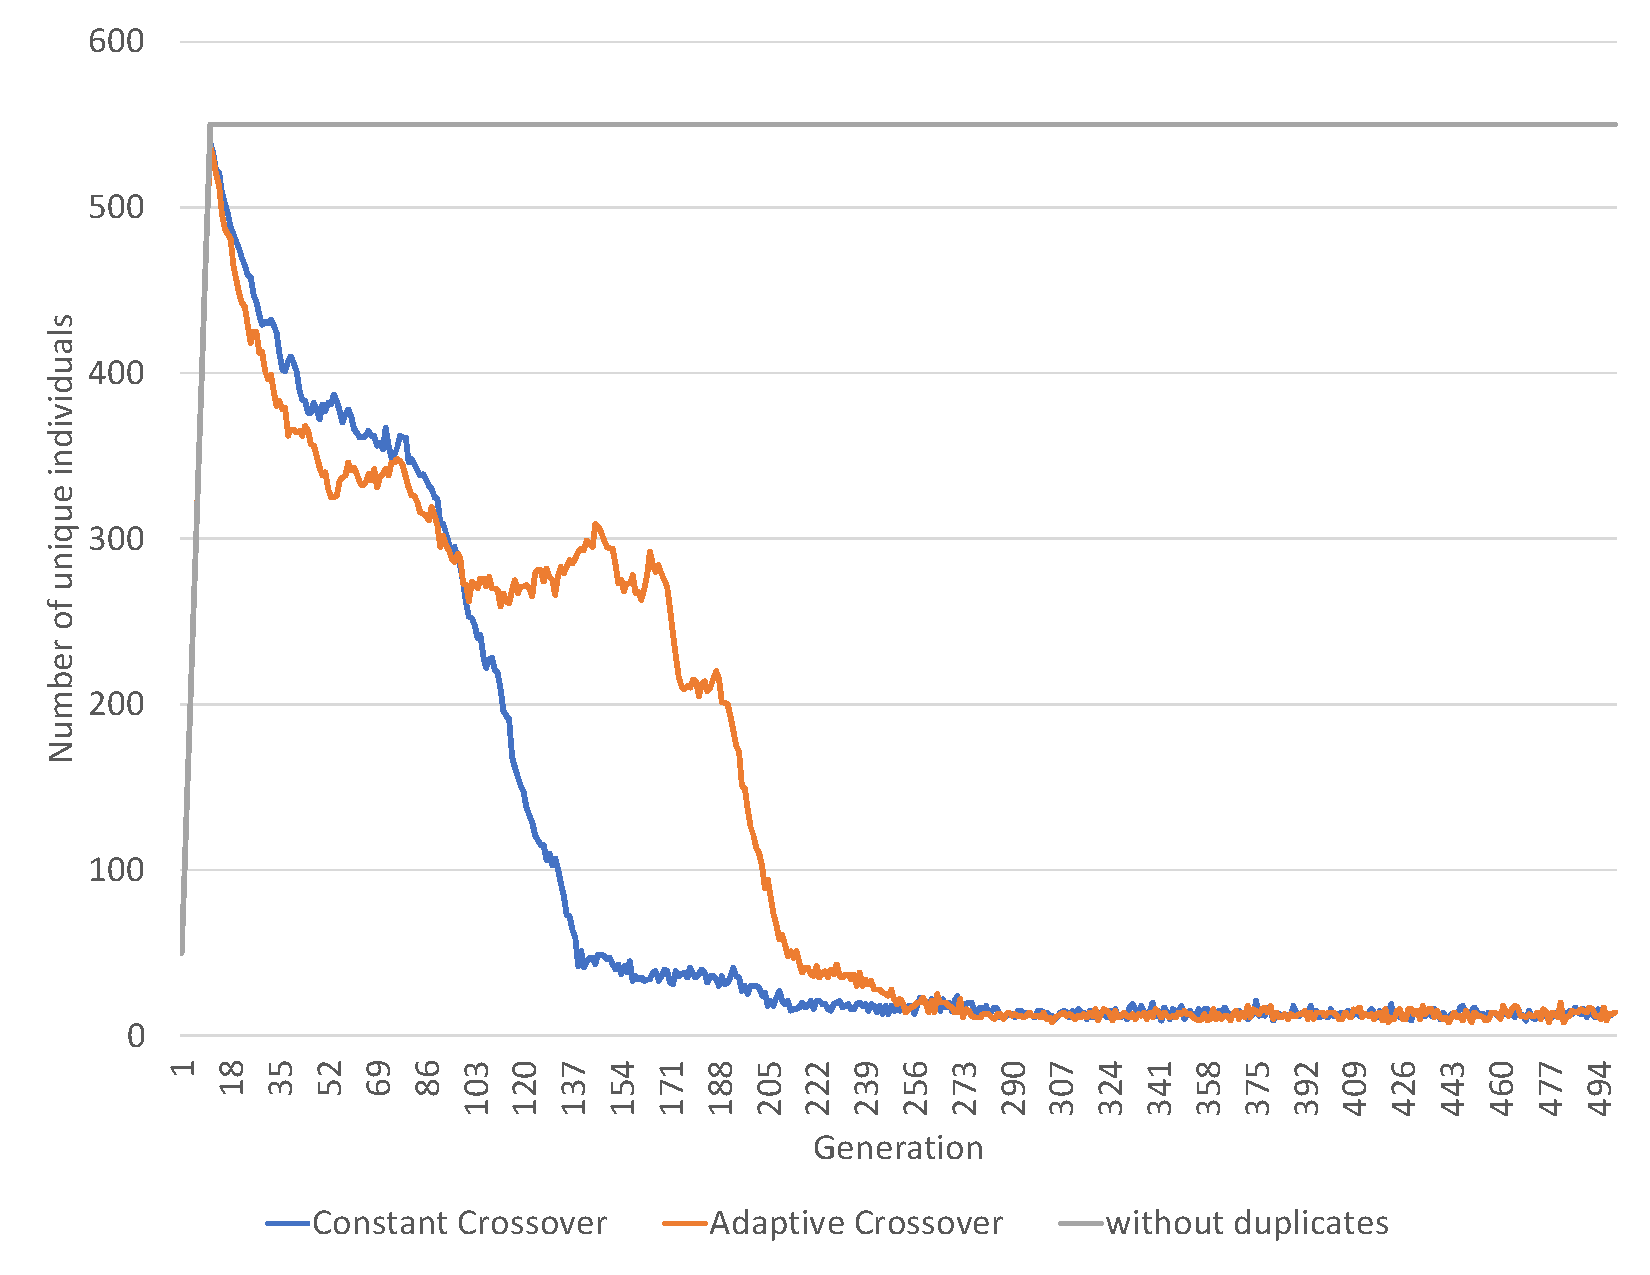
\includegraphics[width=\textwidth]{images/UniqIndividualsPerGeneration3.pdf}
	\caption[]{}
	\label{fig:UniqIndividualsPerGeneration3}
\end{figure}   

The conclusion of this idea is quite pessimistic due to the fact that other approaches work better on this problem, but it may work better than others with different problems or on long term optimization.


